\documentclass[a4paper,oneside,DIV=10,12pt]{scrartcl}

\usepackage{graphicx}
\usepackage{float}

\usepackage{fontspec}
\setmainfont{STIX Two Text}
%\setsansfont{Roboto}
\newfontfamily{\cyrillicfontsf}{Roboto}

\usepackage{microtype}

\usepackage{polyglossia}
\setmainlanguage{ukrainian}

\usepackage{amsmath}
\usepackage{unicode-math}
\setmathfont{STIX Two Math}
\usepackage[retainorgcmds]{IEEEtrantools}

\usepackage{systeme}

\usepackage{booktabs}

\usepackage{siunitx}
\sisetup{output-decimal-marker = {,},
exponent-product = {\cdot}}

\newcommand\schel[1]{\textit{#1}}

\begin{document}
	\begin{titlepage}
		\begin{center}
			Міністерство освіти і науки України\\
			Національний авіаційний університет\\
			Навчально-науковий інститут комп'ютерних інформаційних технологій\\
			Кафедра комп'ютеризованих систем управління
			
			\vspace{\fill}
				Лабораторна робота №2\\
				з дисципліни «Теорія електричних та магнітних кіл»\\
				на тему: «Розрахунок електричного~кола з~експериментальною перевіркою»\\
				Варіант №
				
			\vspace{\fill}
			
			\begin{flushright}
				Виконав:\\
				студент ННІКІТ СП-225\\
				Клокун Владислав\\
				Перевірив:\\
				Молчанов О.~В.
			\end{flushright}
			Київ 2017
		\end{center}
	\end{titlepage}
	
	\section{Мета роботи}
		\begin{enumerate}
			\item Набути необхідні навички практичного розрахунку складного електричного кола постійного струму, використовуючи методу аналізу ланцюгів. Перевірити правильність розрахунку кола, використовуючи рівняння балансу потужності. Побудувати потенціальну діаграму контура.
		\end{enumerate}
		
	\section{Короткі теоретичні відомості}
		Методи розрахунку кіл призначені для визначення струмів в гілках кола, напружень і потужностей на елементах схеми.
		
		Основними методами аналізу ланцюгів, як відомо, є методи рівнянь Кірхгофа (МРК), контурних струмів (МКС), вузлових потенціалів (МВП), еквівалентних перетворень (МЕП).
		
		Схема електричного кола для визначення струмів і потенціалів методом складання систем рівнянь зображена на рис. \ref{fig:schematic}.
		
		\begin{figure}[!htbp]
			\centering
			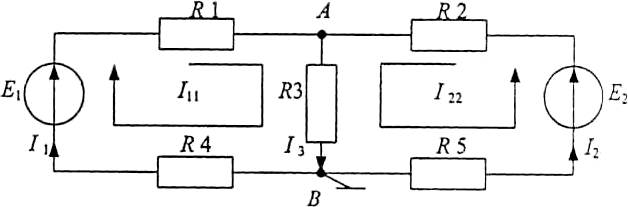
\includegraphics[width=\textwidth]{schematic-01.png}
			\caption{Схема електричного кола}
			\label{fig:schematic}
		\end{figure}
		
		\subsection{Метод рівнянь Кірхгофа}
			Згідно з першим законом Кірхгофа, кількість рівнянь дорівнює кількості вузлів кола мінус одиниця. Згідно з другим законом Кірхгофа, кількість рівнянь дорівнює кількості незалежних контурів системи. В нашому випадку їх три:
			\[
				\begin{cases}
				I_1 + I_2 - I_3 &= U,\\
				I_1R_1 + I_3R_3 + I_1R_4 &= E_1,\\
				I_2R_2 + I_3R_3 + I_2R_2 &= E_2.\\
				\end{cases}
			\]
			
		\subsection{Метод контурних струмів}
			Кількість рівнянь, необхідних для визначення струмів цим методом, дорівнює кількості незалежних контурів. Незалежний контур --- це такий контур, що має хоча б одну гілку, яка не входить в інші контури.
			
			В нашому випадку рівнянь два і вони мають вигляд:
			\[
				\begin{cases}
					I_{11}(R_1 + R_2 + R_4) + I_{22} R_3 = E_1,\\
					I_{11} R_3 + I_{22}(R_2 + R_3 + R_5) = E_2.\\
				\end{cases}
			\]
			
		\subsection{Метод вузлових потенціалів}
			Кількість рівнянь, необхідних для визначення потенціалів, дорівнює кількості вузлів кола мінус одиниця, якщо всі джерела енергії реальні. В нашому випадку рівняння одне:
			\[
				U_A \left( \frac{1}{R_1 + R_4} + \frac{1}{R_3} + \frac{1}{R_2 + R_5} \right) = \frac{E_1}{R_1 + R_4} + \frac{E_2}{R_2 + R_5}.
			\]
			
			Розв'язуючи системи рівнянь будь-яким зручним методом, визначаємо значення струмів або потенціалів. Для методу вузлових потенціалів при визначенні струмів через певні потенціали вузлів необхідно застосовувати узагальнений закон Ома, або як його ще називають «закон Ома для ділянки кола, яка містить джерело ЕРС». З цього всього видно, що найбільш універсальним, але і самим трудомістким методом аналізу кіл є метод рівнянь Кірхгофа, а найбільш ефективними є метод контурних струмів і вузлових потенціалів. Правильність розрахунку кола можна перевірити, використовуючи рівняння балансу потужностей. Алгебраїчна сума потужностей, що виробляються джерелами енергії, дорівнює сумі потужностей, і споживаних резисторами схеми:
			\[
				\sum_{k = 1}^{n} E_k I_k = \sum_{k = 1}^n I^2_k R_k.
			\]
		
	\section{Порядок виконання роботи}
		Використовуючи мультиметр, який знаходиться в лабораторному стенді, а також лабораторний блок №2, виміряти значення опору резисторів \schel{R1} і \schel{R2}, а також напругу нерегульованого джерела ЕРС \schel{$E_2$}. Записати ці значення в табл.~\ref{tab:measurements1}.
		
		\begin{table}[!htbp]
			\centering
			\begin{tabular}{ccccc}
				\toprule
				$E_1, \si{\volt}$ & $E_2, \si{\volt}$ & \schel{R1}, \si{\ohm} & \schel{R2}, \si{\ohm} & \schel{R3}, \si{\ohm} \\
				\midrule
				\num{8,4} & \num{12,8} & \num{78} & \num{76} & \num{168} \\
				\bottomrule
			\end{tabular}
			\caption{Виміри}
			\label{tab:measurements1}
		\end{table}
		
		Розрахувати двома методами, запропонованими викладачем, струми в гілках схеми і напругу на резисторах. Зробити перевірку правильності розрахунку струмів за балансом потужностей. Похибка розрахунку не повинна перевищувати 1\%. Отримані значення занести в табл. \ref{tab:measurements2}.
		
		\subsection{Метод рівнянь Кірхгофа}
			За I законом Кірхгофа кількість рівнянь для вузлів: $2 - 1 = 1$. За II законом Кірхгофа кількість рівнянь для незалежних контурів $3 - (2 - 1) = 2$.
			
			Складаємо систему рівнянь:
			%\[
			%	\left\{
			%\begin{IEEEeqnarray*}{rCrCrCl}
			%	I_1     &+& I_2     &-& I_3     &=& 0\\
			%	R_1 I_1 &-& R_2 I_2 & &         &=& E_1\\
			%	        & & R_2 I_2 &+& R_3 I_3 &=& E_2\\
			%\end{IEEEeqnarray*}
			%	\right.
			%\]
			
			\[
				\begin{cases}
					I_1     + I_2 - I_3     = 0\\
				R_1 I_1 - R_2 I_2           = E_1\\
				          R_2 I_2 + R_3 I_3 = E_2\\
				\end{cases}
			\]
			
			\[
				\begin{cases}
				   I_1 +    I_2 - I_3     = 0\\
				78 I_1 - 76 I_2           = 8{,}4\\
				         76 I_2 + 168 I_3 = 12{,}8\\
				\end{cases}
			\]
			
			Вирішивши систему лінійних алгебраїчних рівнянь, отримаємо $I_1 = -0.01$, $I_2 = -0.12$, $I_3 = 0.13$.
			
		\subsection{Метод контурних струмів}
			\begin{table}[!htbp]
				\centering
				\begin{tabular}{ccccccc}
					\toprule
						Метод розрахунку & \multicolumn{6}{c}{Розрахункові і дослідні значення}\\
							& $I_1, \si{\ampere}$ & $I_2, \si{\ampere}$ & $I_3, \si{\ampere}$ & $U_{\schel{R1}}, \si{\volt}$ & $U_{\schel{R2}}, \si{\volt}$ & $U_{\schel{R3}}, \si{\volt}$ \\
					\midrule
						МРК & & & & & & \\
						МКС & \num{-0.003} & \num{0.053} & \num{0.05} & \num{0.234} & \num{4.028} & \num{8.4}\\
						МВП & & & & & & \\
						Дослідні значення & \num{19e-6} & \num{50,5e-3}& \num{50,5e-3} &\num{0} & \num{4,27} & \num{8,5}\\
						Похибка & & & & & & \\
					\bottomrule
				\end{tabular}
				\caption{Виміри}
				\label{tab:measurements2}
			\end{table}
			
			Зібрати електричну схему експерименту (рис.~\ref{fig:schematic02}), включивши в гілки вимірювальні прилади. Встановити значення опору \schel{R3} і напругу джерела \schel{$E_1$}. Виміряти значення струмів в гілках і напругу на резисторах. Результати досліду занести в табл.~\ref{tab:measurements2}.
			
			\begin{figure}[!htbp]
				\centering
				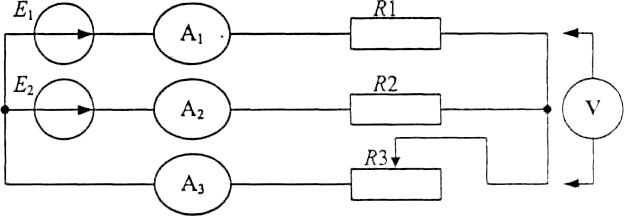
\includegraphics[width=\textwidth]{schematic-02.png}
				\caption{Електрична схема експерименту}
				\label{fig:schematic02}
			\end{figure}
			
			Обчислити похибку розрахунку між дослідними і розрахунковими значеннями і занести результати в табл.~\ref{tab:measurements2}.
			
			Побудувати в масштабі потенціальну діаграму для контура, який містить два джерела ЕРС.
			
			Складаємо систему рівнянь за методом контурних струмів.
			\[
				\begin{cases}
					 I_{11} (R_1 + R_2) - I_{22}  R_2        = E_1 - E_2\\
					-I_{11} R_2         + I_{22} (R_2 + R_3) = E_2\\
				\end{cases}
			\]
			
			\[
				\begin{cases}
					 154 I_{11} -  76 I_{22} = -4{,}4\\
					-76  I_{11} + 244 I_{22} = 12{,}8\\
				\end{cases}
			\]
			
			Розв'язавши систему рівнянь, отримали: $I_{11} = -0{,}003$, $I_{22} = 0{,}05$. Звідси $I_1 = I_{11} = -0{,}003$, $I_2 = -I_{11} + I_{22} = -0{,}053$, $I_1 = I_{22} = -0{,}05$.
		
	\section{Висновки}
		
\end{document}
